\documentclass[12pt]{article}
\usepackage{amsmath, amssymb, amsfonts}
\usepackage{geometry}
\usepackage{tikz}
\usepackage{pgfplots}
\geometry{margin=1in}
\pgfplotsset{compat=1.18}

\title{A Demo Collection of Beautiful Equations and Figures}
\author{Your Name}
\date{\today}

\begin{document}

\maketitle

\section*{Classic Identities}

Euler’s identity:
\[
e^{i\pi} + 1 = 0
\]

Binomial theorem:
\[
(x+y)^n = \sum_{k=0}^n \binom{n}{k} x^{n-k} y^k
\]

\section*{Calculus}

Gaussian integral:
\[
\int_{-\infty}^\infty e^{-x^2}\,dx = \sqrt{\pi}.
\]

\section*{Linear Algebra}

\[
\det\!\begin{bmatrix}
a & b \\
c & d
\end{bmatrix}
= ad - bc
\]

\section*{Series and Limits}

Taylor series of $e^x$:
\[
e^x = \sum_{n=0}^\infty \frac{x^n}{n!}.
\]

\[
\lim_{n\to\infty} \left(1 + \frac{1}{n}\right)^n = e.
\]

\section*{Physics Inspiration}

\begin{align*}
\nabla \cdot \vec{E} &= \frac{\rho}{\varepsilon_0}, \\
\nabla \cdot \vec{B} &= 0, \\
\nabla \times \vec{E} &= -\frac{\partial \vec{B}}{\partial t}, \\
\nabla \times \vec{B} &= \mu_0 \vec{J} + \mu_0\varepsilon_0 \frac{\partial \vec{E}}{\partial t}.
\end{align*}

\section*{TikZ Figures}

\subsection*{1. Venn Diagram (Sets)}

\begin{center}
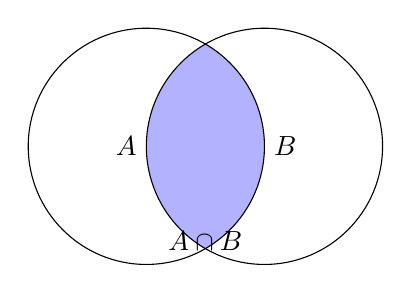
\begin{tikzpicture}
    \begin{scope}
        \clip (0,0) circle(1.5);
        \fill[blue!30] (1.5,0) circle(1.5);
    \end{scope}
    \draw (0,0) circle(1.5) node[left] {$A$};
    \draw (1.5,0) circle(1.5) node[right] {$B$};
    \node at (0.75,-1.2) {$A \cap B$};
\end{tikzpicture}
\end{center}

\subsection*{2. Function Plot}

\begin{center}
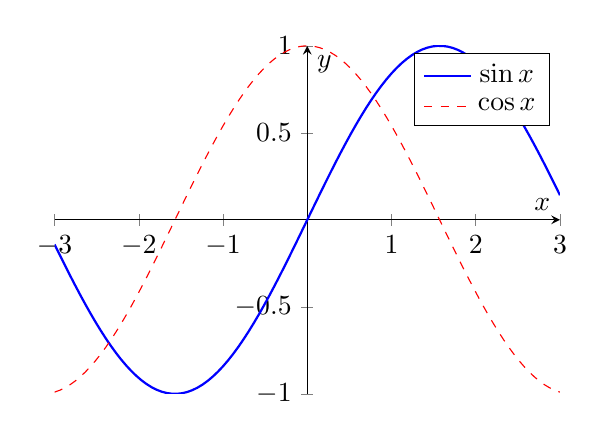
\begin{tikzpicture}
    \begin{axis}[
        axis lines = middle,
        xlabel = $x$,
        ylabel = $y$,
        domain=-3:3,
        samples=100,
        width=8cm,
        height=6cm
    ]
    \addplot[blue, thick] {sin(deg(x))};
    \addplot[red, dashed] {cos(deg(x))};
    \legend{$\sin x$, $\cos x$}
    \end{axis}
\end{tikzpicture}
\end{center}

\end{document}